\begin{tikzpicture}
	\onslide<7->{ \node[] (input_taj) 
		{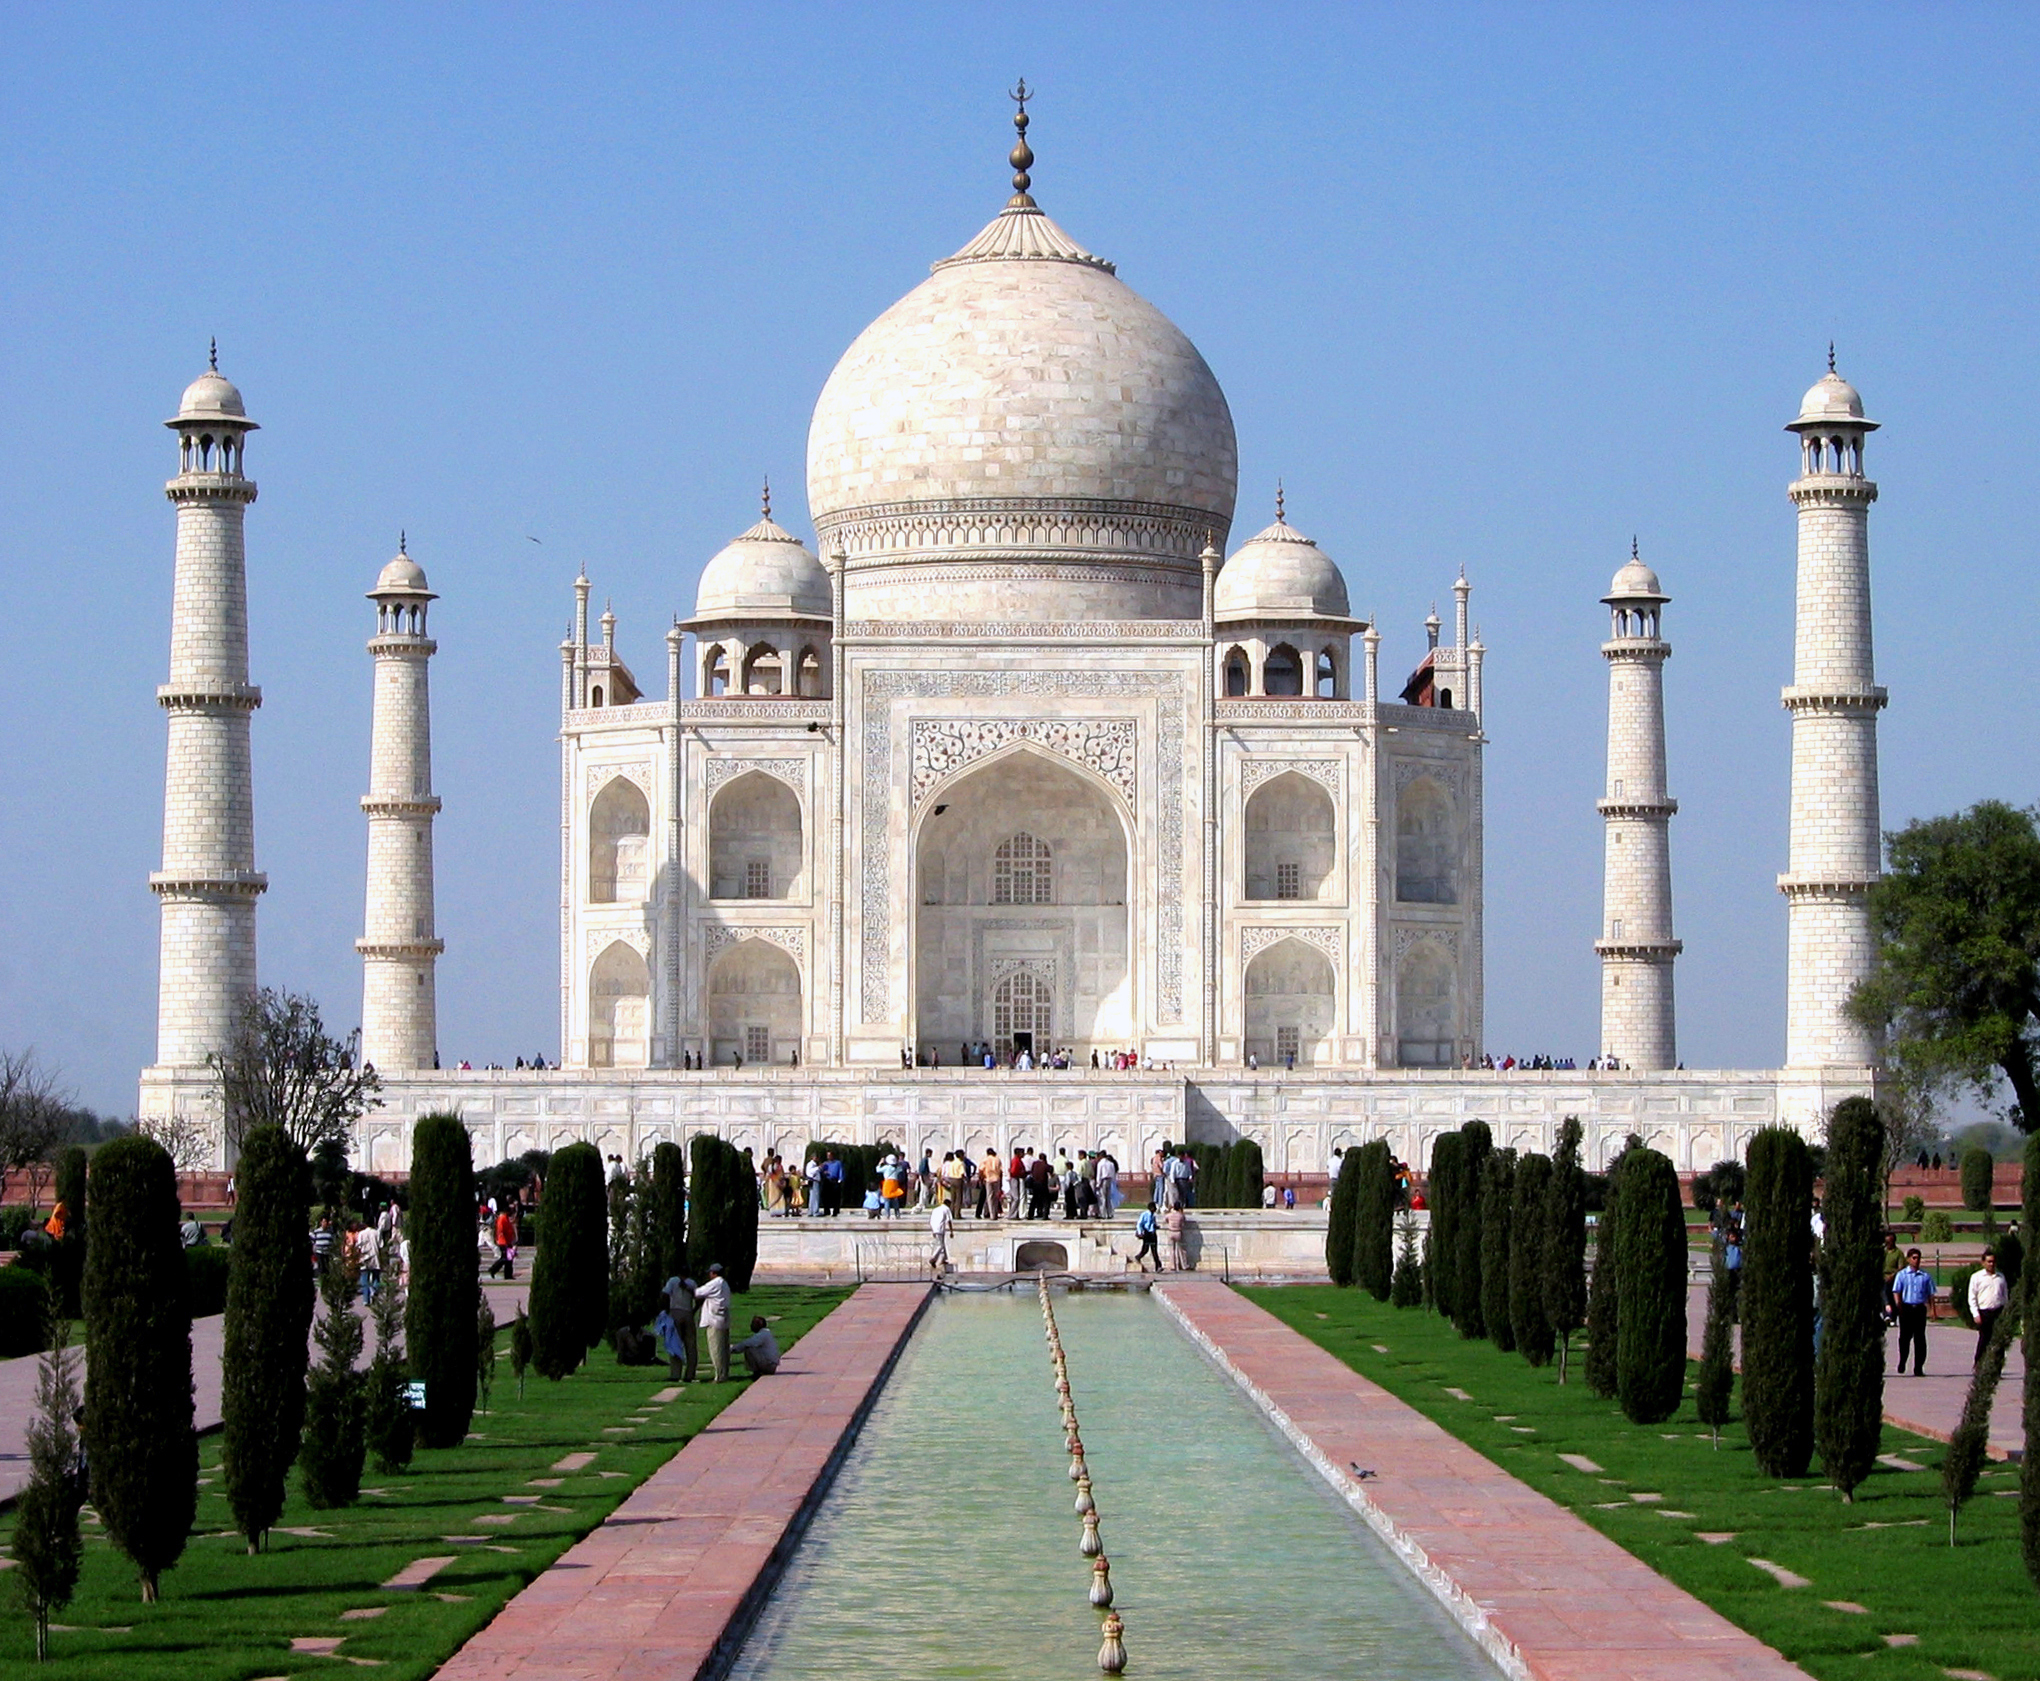
\includegraphics[width=20mm,scale=0.7]{images/taj_mahal.jpg}};}
	\onslide<8->{  \node [right=3cm of input_taj.south,anchor=south west] (sift)  {  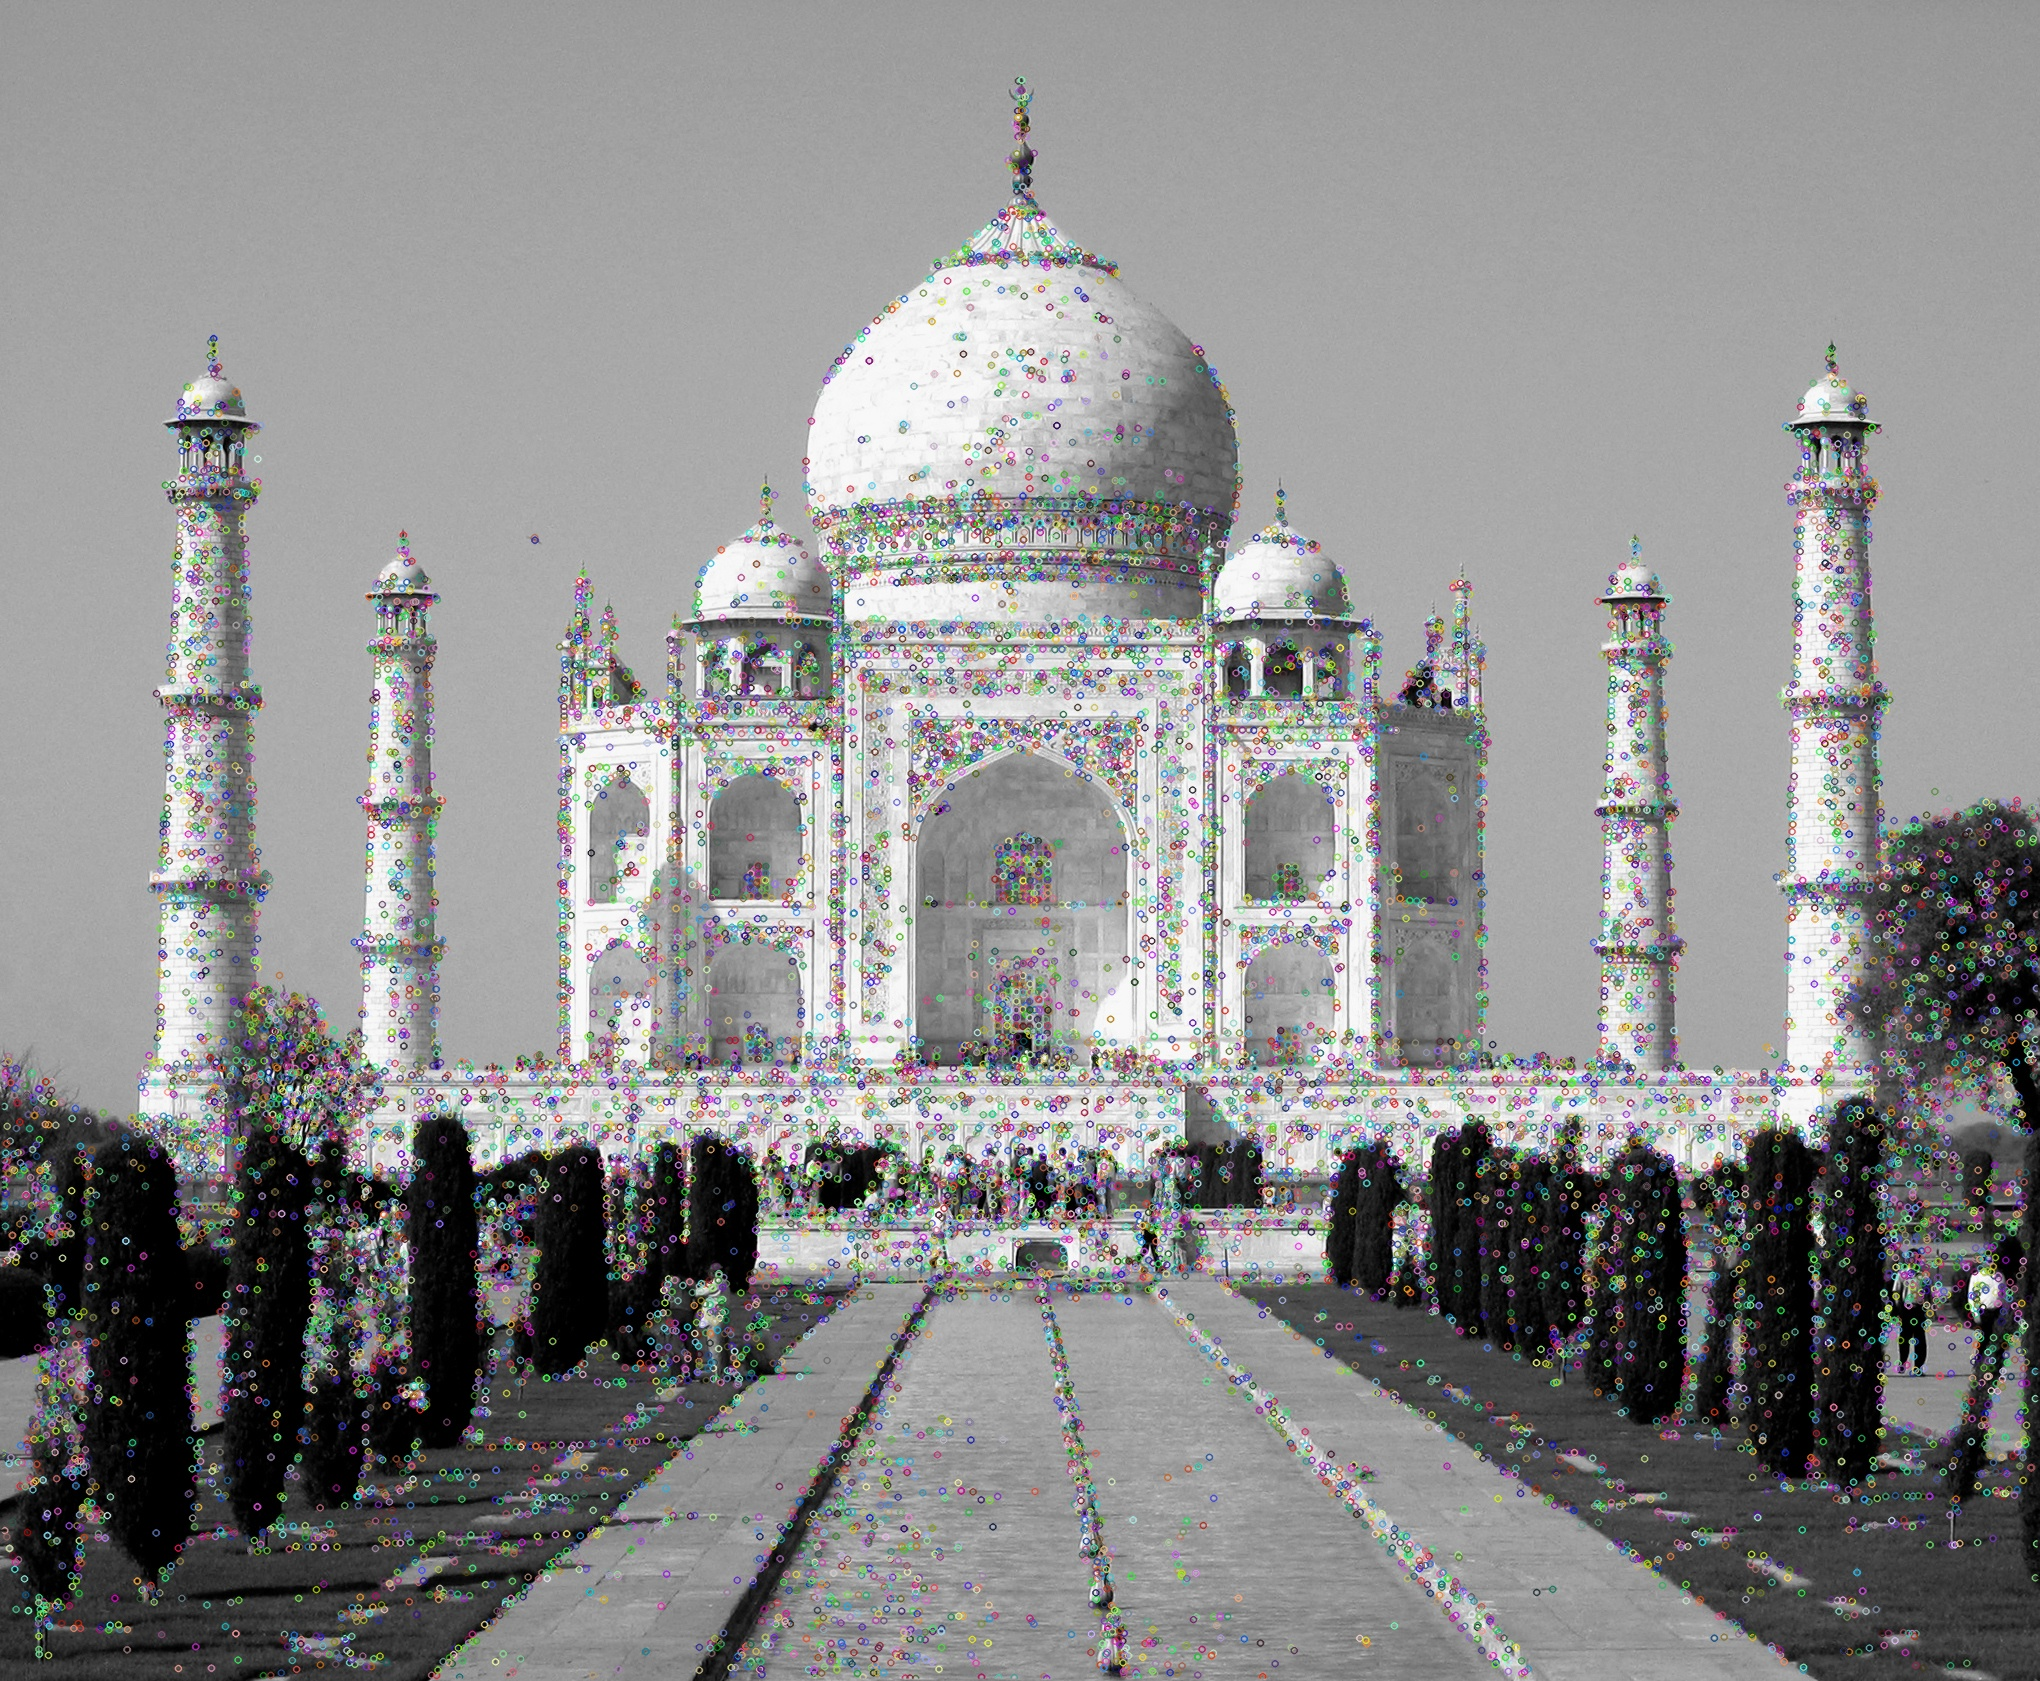
\includegraphics[width=20mm,scale=0.7]{images/SIFT.jpg}};
		\node [right= 0.1cm of sift] (hog)  { 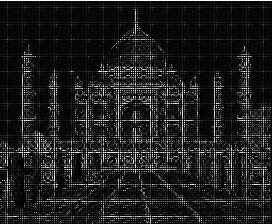
\includegraphics[width=20mm,scale=0.7]{images/hog.jpg}};
		%\node[above of= raw,node distance=1.2cm ] (features)  {Features};
		\draw[->,thick] (input_taj) -- node [name=u,midway, above] {\footnotesize{$SIFT/HOG$}} (sift) ;}
	% \onslide<8->{  \node [right= of hog] (sift)  { 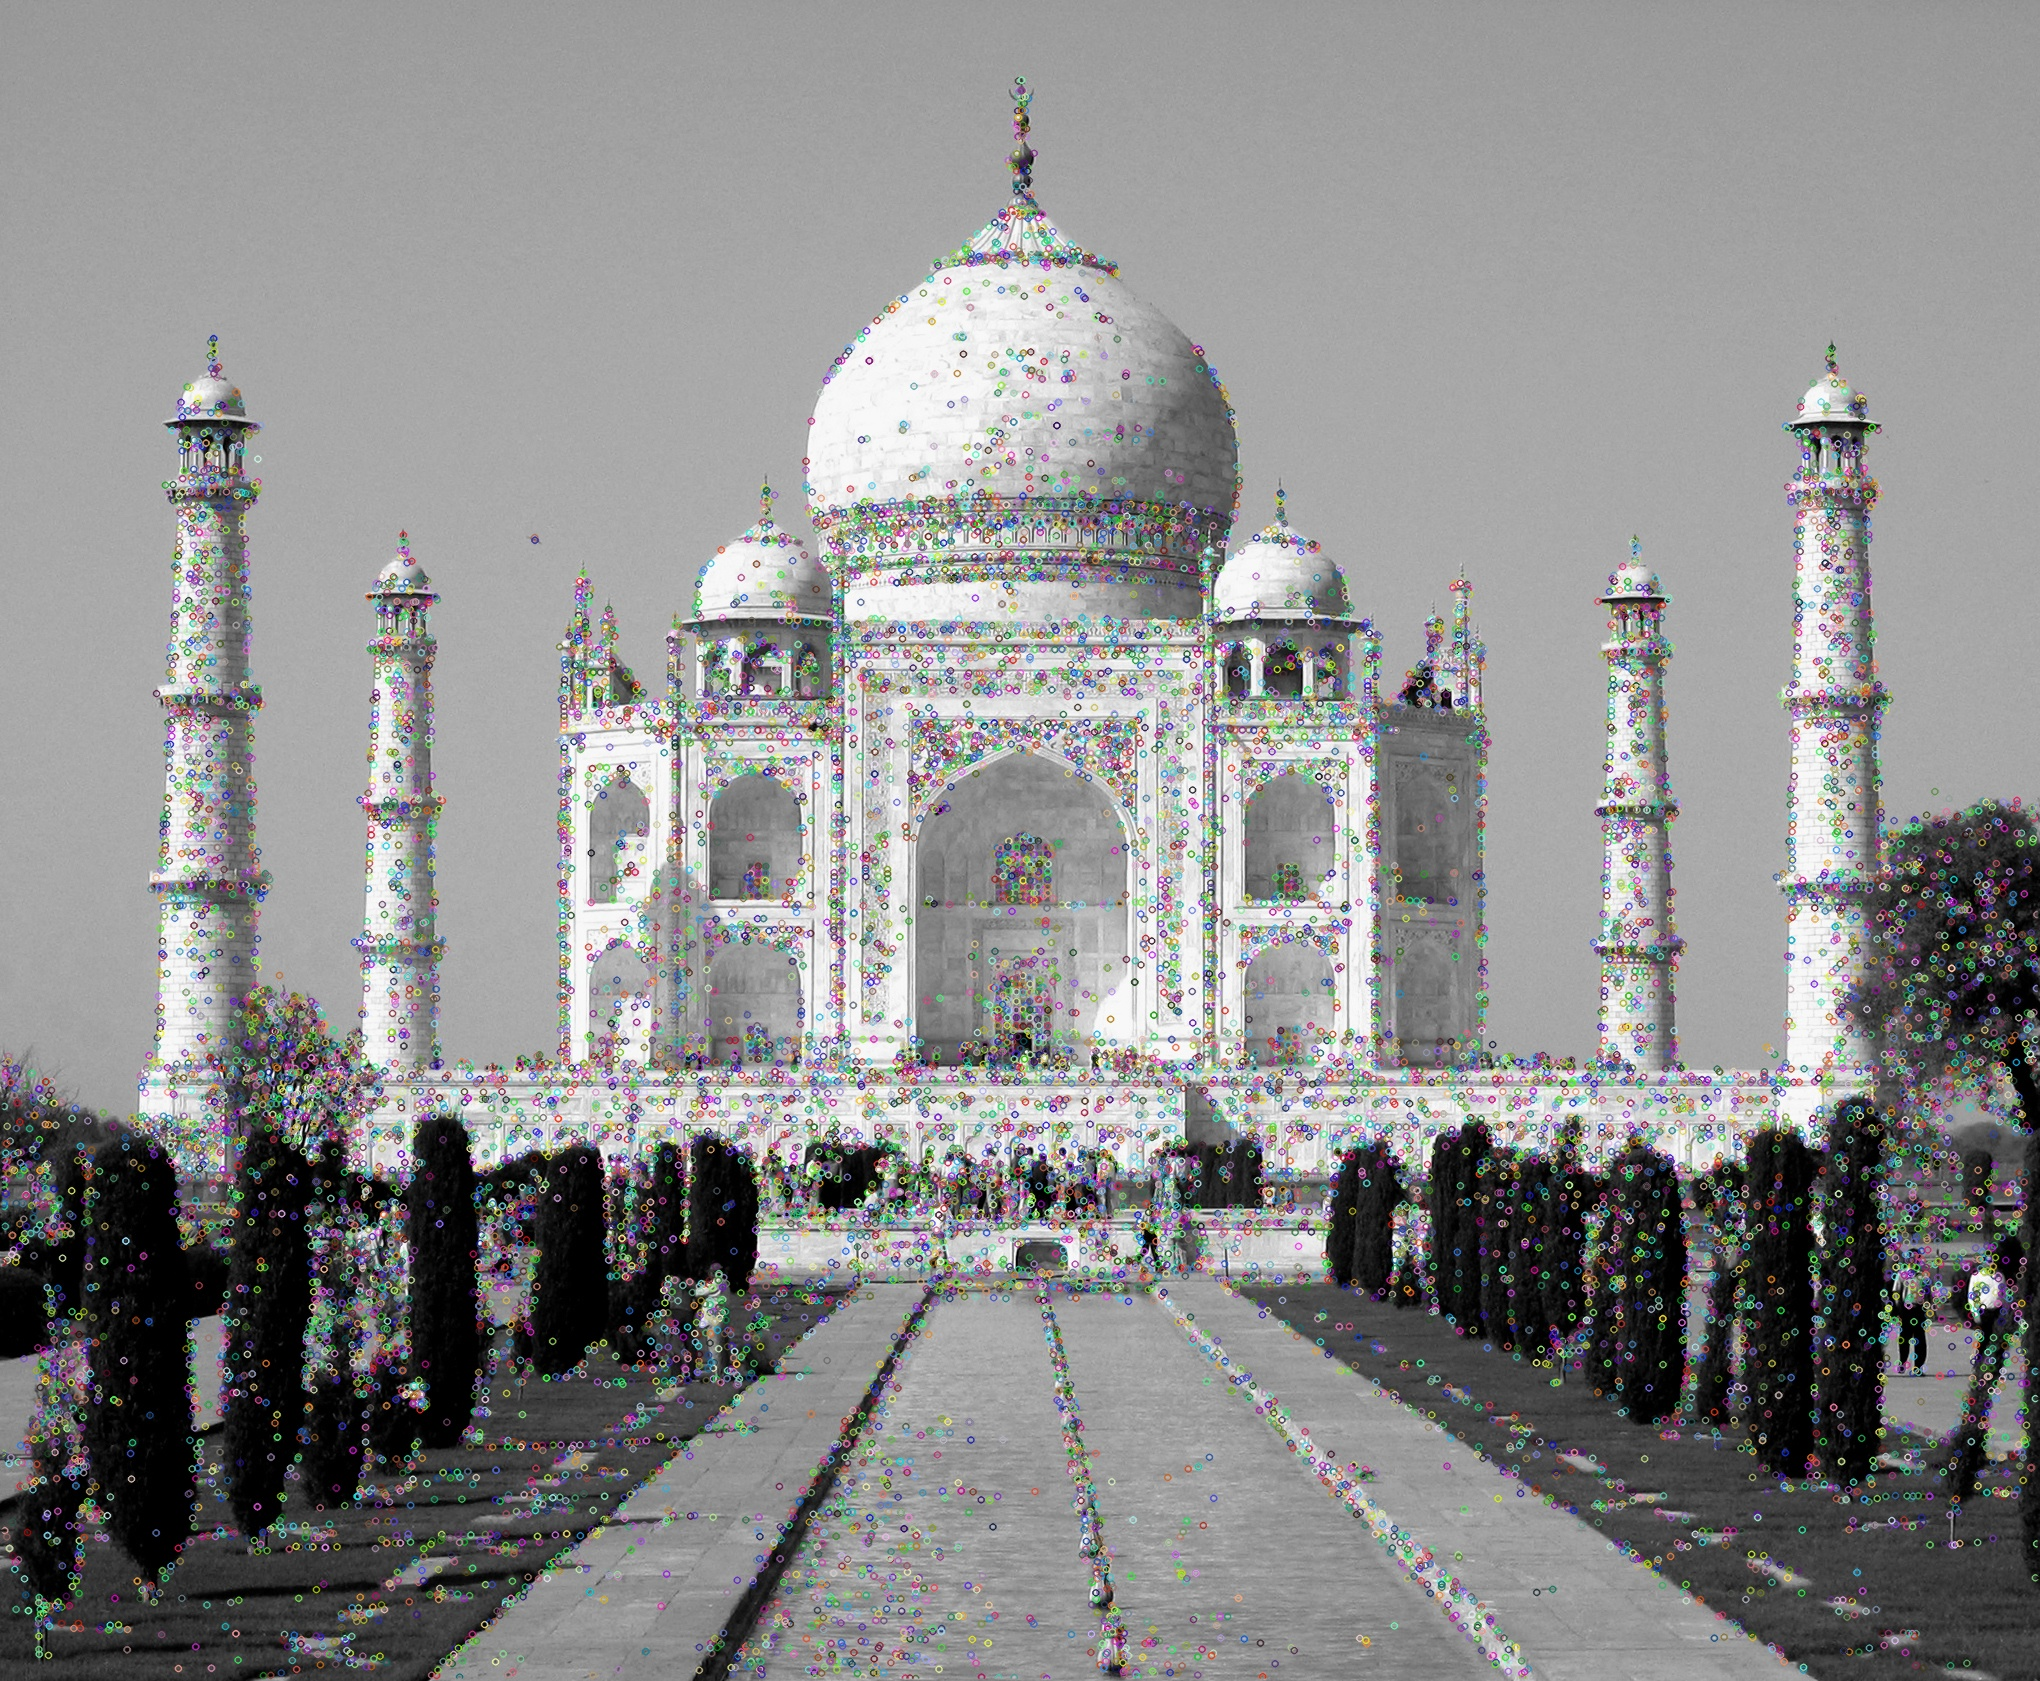
\includegraphics[width=20mm,scale=0.7]{SIFT1.jpg}};
	\onslide<9->{\node [right=4cm of hog.center,anchor= center](output_taj){car, bus, \textcolor{blue}{monument}, flower};
		\draw[->,thick] (hog) -- node [name=v,midway, above]{$ $} (output_taj) ;}

	\onslide<10->{\draw [
			thick,
			decoration={
				brace,
				mirror,
				raise=0.9cm
			},
			decorate
		] (u.south east) -- (hog.east) 
		node [pos=0.5,anchor=north,yshift=-0.9cm,font=\footnotesize] {static feature extraction (no learning)}; 
		\draw [
			thick,
			decoration={
				brace,
				mirror,
				raise=0.9cm
			},
			decorate
		] (v.south east) -- (output_taj.east) 
		node [pos=0.5,anchor=north,yshift=-0.9cm,font=\footnotesize] {learning weights of classifier};
	}
\end{tikzpicture}